\section{Modified Valiant's algorithm}

In this section, we propose how to rearrange the order in which submatrices are processed in the algorithm.
The different order improves the independence of submatrices handling and facilitates the implementation of parallel submatrix processing.

\subsection{Layered submatrices processing}

We propose to divide the parsing table into layers of disjoint submatrices of the same size (see Figure~\ref{fig2}).
Such division is possible because the derivation of a substring of the fixed length does not depend on either left or right contexts.
Each layer consists of square matrices which size is a power of 2.
The layers are computed successively in the bottom-up order.
Each matrix in the layer can be handled independently, which facilitates parallelization of layer processing.

\begin{figure}[h]
\vspace{3mm}
 \begin{center}
 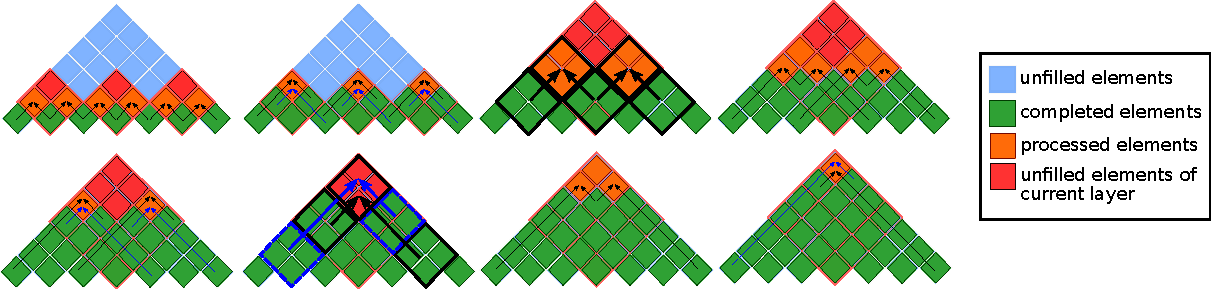
\includegraphics[width=12cm]{pictures/modivis2.pdf}
    \caption{An example of the modification of Valiant's algorithm}
    \label{fig4}
 \end{center}
\vspace{-8mm}
\end{figure}

Figure~\ref{fig4} demonstrates the modified algorithm.
The lowest layer (submatrices of size 1) has already been computed.
The second layer is filled in the steps 1-2.
So the same part of parsing matrix (as in Figure~\ref{fig3}) can be computed only in two steps using parallel computation of submatrix products.

The modified version of Valiant's algorithm is presented in Listing~\ref{algo:modified}.
The procedure \textit{main()} computes the lowest layer $(T_{l, l+1})$, and then divides the table into layers, and computes them with the \textit{completeVLayer()} function.
Thus, \textit{main()} computes all elements of parsing table $T$.

We define \textit{left(subm)}, \textit{right(subm)}, \textit{top(subm)}, \textit{bottom(subm)}, \linebreak \textit{rightgrounded(subm)} and \textit{leftgrounded(subm)} functions which return the submatrices for matrix $\textit{subm} = (l, m, l', m')$ according to the original Valiant's algorithm (Figure~\ref{fig2}).

\begin{algorithm}[h]
\SetAlgoNoLine
\KwIn{$G = (\Sigma, N, R, S), w = a_{1} \dots a_{n}, n \geq 1, n + 1 = 2^p, a_{i} \in \Sigma$ }
\underline{main()}{:}{

 \lFor {$l \in \{1, \ldots, n \}$}{$T_{l, l + 1} = \{A | A \rightarrow a_{l + 1} \in R\}$}
 \For{$1 \le i \le p - 1 $}{
 \textit{layer = constructLayer($i$)}\;
 \textit{completeVLayer(layer)}
 }
 accept if and only if $S \in T_{0, n}$
 \BlankLine
 }

\underline{constructLayer(i)}{:}{
 \BlankLine
 $\{(k2^i, (k+1)2^i, (k + 1)2^i, (k+2)2^i) \, |\, 0 \le k < 2^{p - i} - 1\}$
 \BlankLine
    }
\underline{completeLayer(M)}{:}{
\BlankLine
\If {$\forall (l, m, l', m') \in M \quad (m - l = 1)$}{\lFor{$ (l, m, l', m') \in M$}{$T_{l, l'} = f(P_{l, l'})$}}
\Else{
\textit{completeLayer($\{\textit{bottom(subm)}\, |\,\textit{subm} \in M \})$}\;
\textit{completeVLayer(M)}
}
\BlankLine
}

\underline{completeVLayer(M)}{:}{
 \BlankLine
 $\textit{multiplicationTasks}_1 = \linebreak
    \{\textit{left(subm)}, \textit{leftgrounded(subm)}, \textit{bottom(subm)} \mid \textit{subm} \in M \} \cup \linebreak  \{\textit{right(subm)}, \textit{bottom(subm)}, \textit{rightgrounded(subm)} \mid \textit{subm} \in M\}$\;
 \BlankLine
 \textit{multiplicationTask$_2$} = $\{\textit{top(subm)}, \textit{leftgrounded(subm)}, \textit{right(subm)} \mid \textit{subm} \in M\}$\;
 \BlankLine
 \textit{multiplicationTask$_3$} = $\{\textit{top(subm)}, \textit{left(subm)}, \textit{rightgrounded(subm)} \mid \textit{subm} \in M\}$\;
 \BlankLine
 \textit{performMultiplications(multiplicationTask$_1$)}\;
 \textit{completeLayer($\{\textit{left(subm)} \mid subm \in M \} \cup \{\textit{right(subm)} \mid \textit{subm} \in M \}$)}\;
 \textit{performMultiplications(multiplicationTask$_2$)}\;
 \textit{performMultiplications(multiplicationTask$_3$)}\;
 \textit{completeLayer($\{top(subm) \mid subm \in M \}$)}

 }
 \BlankLine

 \underline{performMultiplication(tasks)}{:}{\\
 \lFor{$ (m, m1, m2) \in \textit{tasks}$}{$P_{m} = P_{m} \cup (T_{m1} \times T_{m2})$}
 }

\caption{Parsing by Matrix Multiplication: Modified Version}
\label{algo:modified}
\end{algorithm}

The procedure \textit{completeVLayer(M)} takes an array of disjoint submatrices $M$ which represents a layer.
For each \textit{subm = (l, m, l', m') $\in M$} this procedure computes \textit{left(subm), right(subm), top(subm)}.
The procedure assumes that the elements of \textit{bottom(subm)} and $T_{i, j}$ for all $i$ and $j$ such that $l \leq i < j < m$ and $  l' \leq i < j < m'$ are already constructed.
Also it is assumed that the current value of
$P_{i, j} =  \{ (B, C) \mid \exists k, (m \le k < l'), a_{i + 1} \dots a_{k} \in L_G(B), a_{k + 1} \dots a_{j} \in L_G(C)\} $ for all $i$ and $j$ such that $l \leq i < m$ and $l' \leq j < m'$.

The procedure \textit{completeLayer(M)} takes an array of disjoint submatrices $M$, but unlike the previous one, it computes $T_{i, j}$ for all $(i, j) \in subm$.
This procedure requires the same assumptions on $T_{i, j}$  and $P_{i, j}$  as in the original algorithm.

In other words, \textit{completeVLayer(M)} computes the entire layer \textit{M} \linebreak and \textit{completeLayer($M_{2}$)} is a helper function which is necessary for computation of smaller square submatrices $subm_{2} \in M_{2}$, where $M_2$ is a sublayer of \textit{M}.

Finally, the procedure \textit{performMultiplication(tasks)}, where \textit{tasks} is an array of triples of submatrices, performs the basic step of the algorithm: matrix multiplication.
It is worth mentioning that $|tasks| \ge 1$ and each task can be computed independently, while the original algorithm handles one \textit{task} per step sequentially.
So, the practical implementation of this procedure can easily utilize different techniques of parallel array processing.

\subsection{Correctness and complexity}

We provide the proof of correctness and time complexity of the proposed modification in this section.

\begin{lemma}
Let $M$ be a layer. If for all $(l, m, l', m') \in M$:
\begin{enumerate}
  \item $T_{i, j} = \{ A \mid  a_{i + 1} \dots a_{j} \in L_G(A)\}$ for all $i$ and $j$ such that $l \leq i < j < m$ and $l' \leq i < j < m'$;
  \item $P_{i, j} =  \{ (B, C) \mid \exists k, (m \le k < l'): a_{i + 1} \dots a_{k} \in L_G(B), a_{k + 1} \dots a_{j} \in L_G(C)\}$ for all $l \leq i < m$ and $l' \leq j < m'$.
\end{enumerate}

Then the procedure \textit{completeLayer(M)}, returns correctly computed sets of $T_{i, j}$ for all $l \leq i < m$ and $l' \leq j < m'$ for all $(l, m, l', m') \in M$.
\end{lemma}

\begin{proof}

The algorithm from listing~\ref{algo:modified} is given by mutually recursive functions \textit{completeLayer()} and \textit{completeVLayer()}. Next we show, that if all necessary conditions are met, \textit{completeVLayer(M)} return correctly computed layer $M$.

We consider the matrix of size $m - l = 1$ (and then the elements of layer $M$ are correctly computed in lines 10-11) and thereafter the lemma can be proved by induction by $m - l$.


\end{proof}

\begin{theorem}
Algorithm from listing~\ref{algo:modified} correctly computes $T_{i, j}$ for all i and j, thus an input string $a = a_{1}a_{2} \dots a_{n} \in L_{G}(S)$ if and only if $S \in T_{0, n}$.
\end{theorem}

\begin{proof}
Primarily to prove the theorem, we show by induction that all layers of the parsing table T are computed correctly.

\underline{\textbf{Basis:}} layer of size $1 \times 1$.
Parsing table \textit{T} consists of one layer of size 1 and its elements are correctly computed in lines 2-3 in listing~\ref{algo:modified}.

\underline{\textbf{Inductive step:}} assume any layer of size less than or equal to $2^{r - 2} \times 2^{r - 2}$ are computed correctly. 

Define layer of size $2^{r - 1} \times 2^{r - 1}$ as M. 
Hereinafter \textit{subm = (l, m, l', m')} is a typical element of layer M.

Consider \textit{completeVLayer(M)} call. 

Firstly, \textit{performMultiplications(multiplicationTask$_1$)} adds to each P$_{i,j}$ all pairs 
$(B, C)$ such that $\exists k$, $(\frac{l+m}{2} \le k < l')$, $a_{i + 1} \dots a_{k} \in L_{G}(B)$, $a_{k + 1} \dots a_{j} \in L_{G}(C)$ for all $(i, j)$ $\in leftsublayer(M)$
and
$(B, C)$ such that $\exists k$, $(m \le k < \frac{l'+m'}{2})$, $a_{i + 1} \dots a_{k} \in L_{G}(B)$, $a_{k + 1} \dots a_{j} \in L_{G}(C)$ for all $(i, j)$ $\in rightsublayer(M)$.
Now \textit{completeLayer(leftsublayer(M) $\cup$ rightsublayer(M))} can be called and it returns correctly computed \textit{leftsublayer(M) $\cup$ rightsublayer(M)}.

Then \textit{performMultiplications} called with arguments 
\textit{multiplicationTask$_2$} and \textit{multiplicationTask$_3$} adds pairs 
$(B, C)$ such that $\exists k$, $(\frac{l+m}{2} \le k < m)$, $a_{i + 1} \dots a_{k} \in L_{G}(B)$, $a_{k + 1} \dots a_{j} \in L_{G}(C)$ 
and pairs
$(B, C)$ such that $\exists k$, $(l' \le k < \frac{l'+m'}{2})$, $a_{i + 1} \dots a_{k} \in L_{G}(B)$, $a_{k + 1} \dots a_{j} \in L_{G}(C)$
to each element P$_{i,j}$ for all $(i, j)$ $\in topsublayer(M)$. 
So as $m = l'$ (from the construction of the layer), condition for elements of matrix $P$ are fulfilled.
Now \textit{completeLayer(topsublayer(M))} can be called and it returns correctly computed \textit{topsublayer(M)}.

All $T[i, j]$ $\forall (i, j) \in M$ are computed correctly.

Thus, \textit{completeVLayer(M)} returns correct $T_{i, j}$ for all $(i, j)$ $\in M$ for any layer M of parsing table T and lines 4-6 in listing~\ref{algo:modified} return all $T_{i, j} =  \{ A \mid A \in N, $ $a_{i + 1} \dots a_{j} \in L_{G}(A)\}$.
\end{proof}


\begin{lemma}
Let \textit{calls$_{r}$} is a number of the calls of \textit{completeVLayer(M)} where for all $(l, m, l', m') \in M$ with $m - l = 2^{p - r}$.
\begin{itemize}
 \item for all $r \in \{ 1, .., p - 1\}$  $\sum_{n=1}^{calls_r}{|M|}$ is exactly $2^{2r - 1} - 2^{r - 1}$;
 \item for all $r \in \{ 1, .., p - 1\}$ products of submatrices of size $2^{p - r} \times 2^{p - r}$ are calculated exactly $2^{2r - 1} - 2^{r}$ times.
\end{itemize}
\end{lemma}

\begin{proof}

Prove the first statement by induction on $r$.

\underline{\textbf{Basis:}} $r = 1$. \textit{calls$_{1}$} and $|M| = 1$. So, $2^{2r - 1} - 2^{r - 1} = 2^1 - 2^0 = 1$.

\underline{\textbf{Inductive step:}} assume that $\sum_{n=1}^{calls_r}{|M|}$ is exactly $2^{2r - 1} - 2^{r - 1}$ for all $r \in \{ 1, .., q\}$.

Let us consider $r = q + 1$.

Firstly, note that function $\textit{costructLayer(r)}$ returns $2^{p - r} - 1$ matrices of size $2^r$, so in the call of \textit{completeVLayer(costructLayer(p - r))}  \textit{costructLayer(p - r)} returns $2^r - 1$ matrices of size $2^{p - r}$. 
Secondly, \textit{completeVLayer()} is called 3 times for the left, right and top submatrices of size $2^{p - (r - 1)}$. Finally, \textit{completeVLayer()} is called 4 times for the bottom, left, right and top submatrices of size $2^{p - (r - 2)}$, except $2^{r - 2} - 1$ matrices which were already computed.

Then, $\sum_{n=1}^{calls_r}{|M|} = 2^{r} - 1 + 3 \times (2^{2(r - 1) - 1} - 2^{(r - 1) - 1}) + 4 \times (2^{2(r - 2) - 1} - 2^{(r - 2) - 1}) - (2^{r - 2} - 1) = 2^{2r - 1} - 2^{r - 1}$.

Now we know $\sum_{n=1}^{calls_{r-1}}{|M|}$  is $2^{2(r - 1) - 1} - 2^{(r - 1) - 1}$ and we can calculate the number of products of submatrices of size $2^{p - r} \times 2^{p - r}$. 
During these calls \textit{performMultiplications} runs 3 times, $|multiplicationTask1| = 2 \times 2^{2(r - 1) - 1} - 2^{(r - 1) - 1}$ and $|multiplicationTask2|$ = $|multiplicationTask3| = 2^{2(r - 1) - 1} - 2^{(r - 1) - 1}$. So, the number of products of submatrices of size $2^{p - r} \times 2^{p - r}$ is $ 4 \times (2^{2(r - 1) - 1} - 2^{(r - 1) - 1}) = 2^{2r - 1} - 2^{r}$.
\end{proof}

\begin{theorem}
Let $|G|$ be a length of the description of the grammar G and let n be a length of an input string. Then algorithm from listing~\ref{algo:modified} calculates matrix \textit{T} in $\mathcal{O}(|G|BMM(n)\log{n})$ where BMM(n) is the number of operations needed to multiply two Boolean matrices of size $n \times n$.
\end{theorem}

\begin{proof}
The proof is almost identical with the proof of theorem 1 given by Okhotin~\cite{Okhotin:2014:PMM:2565359.2565379}, because, as shown in the last lemma, the Algorithm 1 has the same number of products of submatrices.
\end{proof}

To summarize, the correctness of the modification was proved and it was shown that the time complexity remained the same as in Valiant's version.


\subsection{Algorithm for substrings}

Next, we show how our modification can be applied to the string-matching problem.
To find all substrings of size $s$, which can be derived from a start symbol for an input string of size $n = 2^p - 1$, we need to compute layers with submatrices of size not greater than $2^{r}$, where $2^{r - 2} < s \le 2^{r - 1}$.

Let $r = p - (m - 2)$ and consequently $(m - 2) = p - r$.
For any  $m \le i \le p$ products of submatrices of size $2^{p - i}$ are calculated exactly $2^{2i - 1} - 2^{i}$ times and each of them imply multiplying $C = \mathcal{O}(|G|)$ Boolean submatrices. Let $\mathrm{BMM} = n^\omega f(n)$, where $\omega \geq 2$ and $f(n) = n^{o(1)}$.
Now we estimate the number of operations needed to find all substrings:

\begin{equation*}
\begin{array}{c}
C \cdot \sum\limits_{i=m}^p 2^{2i - 1} \cdot 2^{\omega(p - i)} \cdot f(2^{p - i}) =
C \cdot 2^{\omega r}\sum\limits_{i=2}^{r} 2^{(2 - \omega)i} \cdot 2^{2(p - r) - 1} \cdot f(2^{r - i}) \le \\
C \cdot 2^{\omega r} f(2^{r}) \cdot 2^{2(p - r) - 1} \sum\limits_{i=2}^{r} 2^{(2 - \omega)i} =
\mathrm{BMM}(2^{r}) \cdot 2^{2(p - r) - 1} \sum\limits_{i=2}^{r} 2^{(2 - \omega)i}
\end{array}
\end{equation*}

Thus, time complexity for searching all substrings of size not greater than $2^{r}$ is $O(2^{2(p - r) - 1}|G|\mathrm{BMM}(2^{r})(r - 1))$ where the appeared factor meet the number of matrices in the last completed layer, while time complexity for the full input string is $O(|G|\mathrm{BMM}(2^p)(p - 1))$. 
The Valiant's algorithm completely calculate at least 2 triangle submatrices of size $\frac{n}{2}$, as shown in Figure~\ref{fig5}, thus the minimum asymptotic complexity is $O(|G|\mathrm{BMM}(2^{p - 1})(p - 2))$.
Thus we can conclude that the modification is asymptotically faster than the original algorithm for substrings of size $s \ll n$.

\begin{figure}
\vspace{3mm}
 \begin{center}
 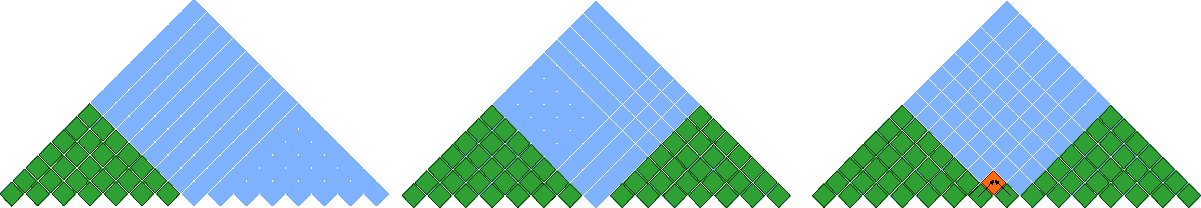
\includegraphics[width=12cm]{pictures/valsubstring.pdf}
    \caption{The number of elements necessary to compute in Valiant's algorithm. It is necessary to calculate at least 2 triangle submatrices of size $\frac{n}{2}$.}
    \label{fig5}
 \end{center}
\vspace{-8mm}
\end{figure}
